%%%%%%%%%%%%%%%%%%%%%%%%%%%%%%%%%%%%%%%%%%%%%%%%%%%%%%%%%%%%%%%%%%%%%%%%%%%%%%%%%%
\begin{frame}[fragile]\frametitle{}
\begin{center}
{\Large Introduction}
\end{center}
\end{frame}

%%%%%%%%%%%%%%%%%%%%%%%%%%%%%%%%%%%%%%%%%%%%%%%%%%%%%%%%%%%%%%%%%%%%%%%%%%%%%%%%%%
\begin{frame}[fragile]\frametitle{Future AI?}
  \begin{itemize}
    \item What are future AI applications like?
	\begin{itemize}
		\item Generative: Generate content like text \& image
		\item Agentic: Execute complex tasks on behalf of human
	 \end{itemize}
	\item How do we empower every developer to build them?: 
	\begin{itemize}
		\item Co-Pilots
		\item Autonomous
	 \end{itemize}	
  \end{itemize}
\end{frame}

%%%%%%%%%%%%%%%%%%%%%%%%%%%%%%%%%%%%%%%%%%%%%%%%%%%%%%%%%%%%%%%%%%%%%%%%%%%%%%%%%%
\begin{frame}[fragile]\frametitle{Introduction to AI Agents}
    \begin{itemize}
        \item 2024 is expected to be the year of AI agents.
        \item AI agents combine multiple components to solve complex problems.
        \item Shifting from monolithic models to compound AI systems.
        \item Compound AI systems use system design for better problem solving.
        \item AI agents improve with reasoning, acting, and memory components. (ReAct = Reasoning + Acting)
    \end{itemize}
\end{frame}

%%%%%%%%%%%%%%%%%%%%%%%%%%%%%%%%%%%%%%%%%%%%%%%%%%%%%%%%%%%%%%%%%%%%%%%%%%%%%%%%%%
\begin{frame}[fragile]\frametitle{What is an Agent?}
    \begin{itemize}
        \item Agent acts, take you from one state to the other state, provides value by workflow automation. (ReAct paper: Reasoning and Action), it can plan and make decisions.
		\item Agents have access to tools (ToolFormer paper) e.g. Search APIs, booking, send email etc.
		\item Interacting of external environment and other Agents, etc.
		\item Memory to keep the history of conversations/actions done so far.
		\item May have human-in-loop to keep it sane in the wild-world.
		\item Agents were there from 1950's but they are effective because of LLMs.
    \end{itemize}
\end{frame}

%%%%%%%%%%%%%%%%%%%%%%%%%%%%%%%%%%%%%%%%%%%%%%%%%%%%%%%%%%%%%%%%%%%%%%%%%%%%%%%%%%
\begin{frame}[fragile]\frametitle{What are Agents?}
    \begin{itemize}
        \item Agents are systems where LLMs dynamically direct their own processes and tool usage
        \item Can operate autonomously over extended periods using various tools
        \item Distinct from workflows: agents have dynamic control vs. predefined code paths
        \item Essential component in modern AI systems with varying degrees of autonomy
    \end{itemize}
\end{frame}

%%%%%%%%%%%%%%%%%%%%%%%%%%%%%%%%%%%%%%%%%%%%%%%%%%%%%%%%%%%%%%%%%%%%%%%%%%%%%%%%%%
\begin{frame}[fragile]\frametitle{What Are LLM Agents?}
\begin{columns}
    \begin{column}[T]{0.6\linewidth}
      \begin{itemize}
        \item LLMs predict the next token in a sequence—no memory.
        \item Conversations are simulated by sampling many tokens.
        \item LLMs struggle with tasks like basic arithmetic.
        \item Augmented LLMs use tools and memory to enhance capabilities.
        \item An Agent perceives and acts upon its environment.
        \item Agentic LLMs use text as input (sensor) and tools as actuators.
        \item Planning and reasoning enable agent-like behavior.
        \item LLM Agents vary in autonomy based on system design.
      \end{itemize}
    \end{column}
    \begin{column}[T]{0.4\linewidth}
        \begin{center}
        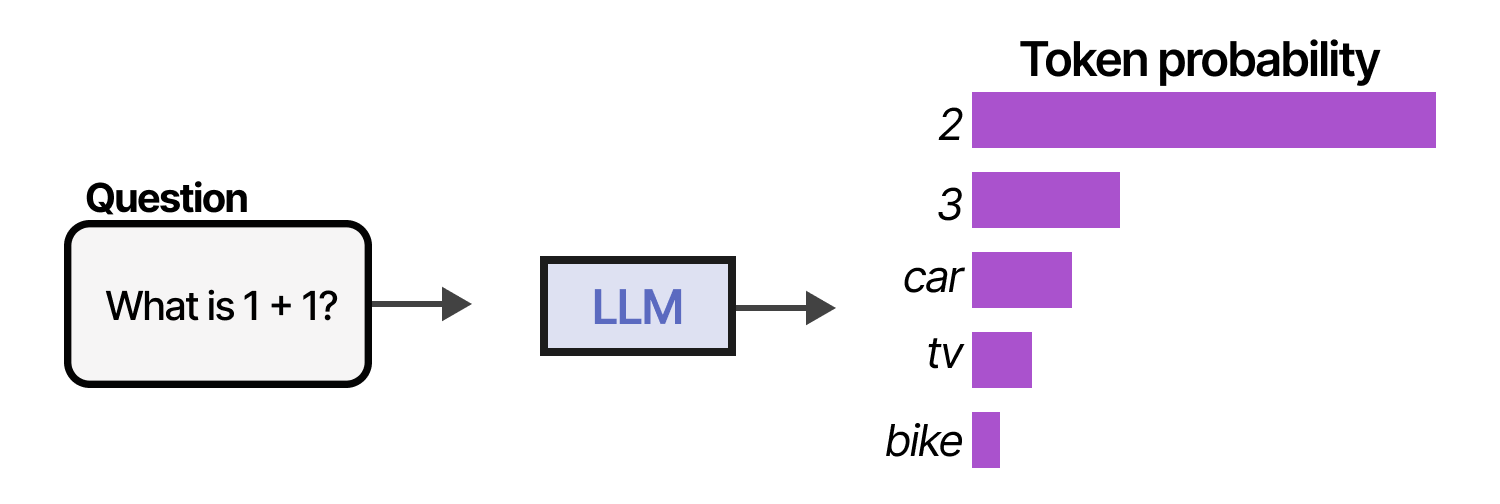
\includegraphics[width=0.8\linewidth,keepaspectratio]{aiagents92}
		
        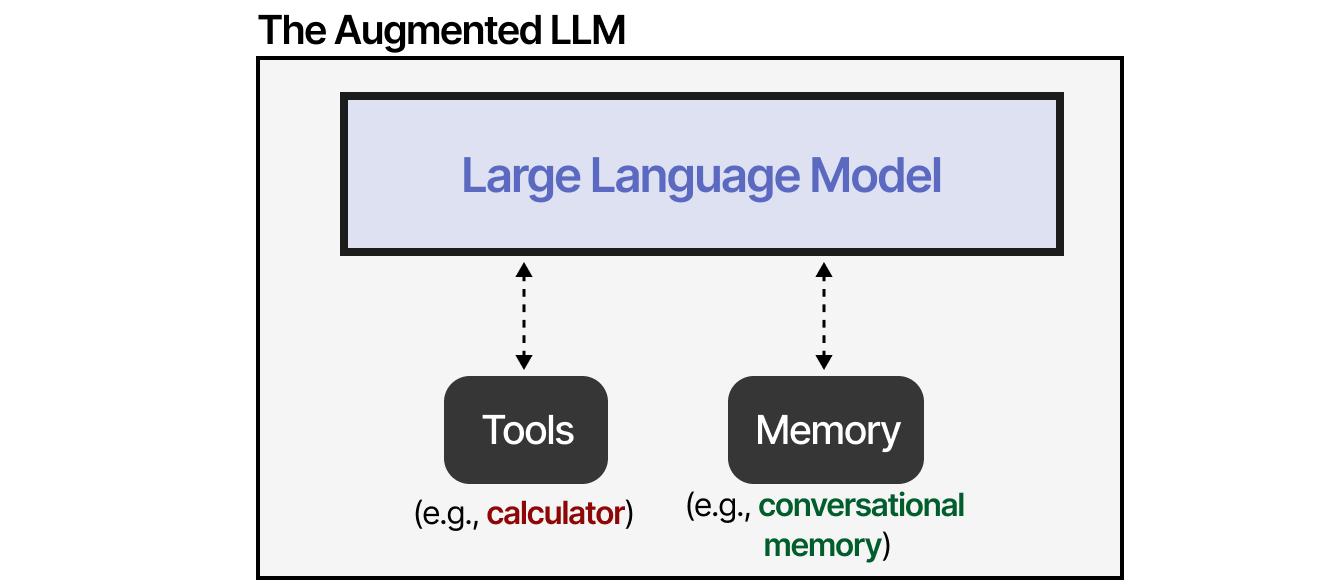
\includegraphics[width=0.8\linewidth,keepaspectratio]{aiagents93}
		
        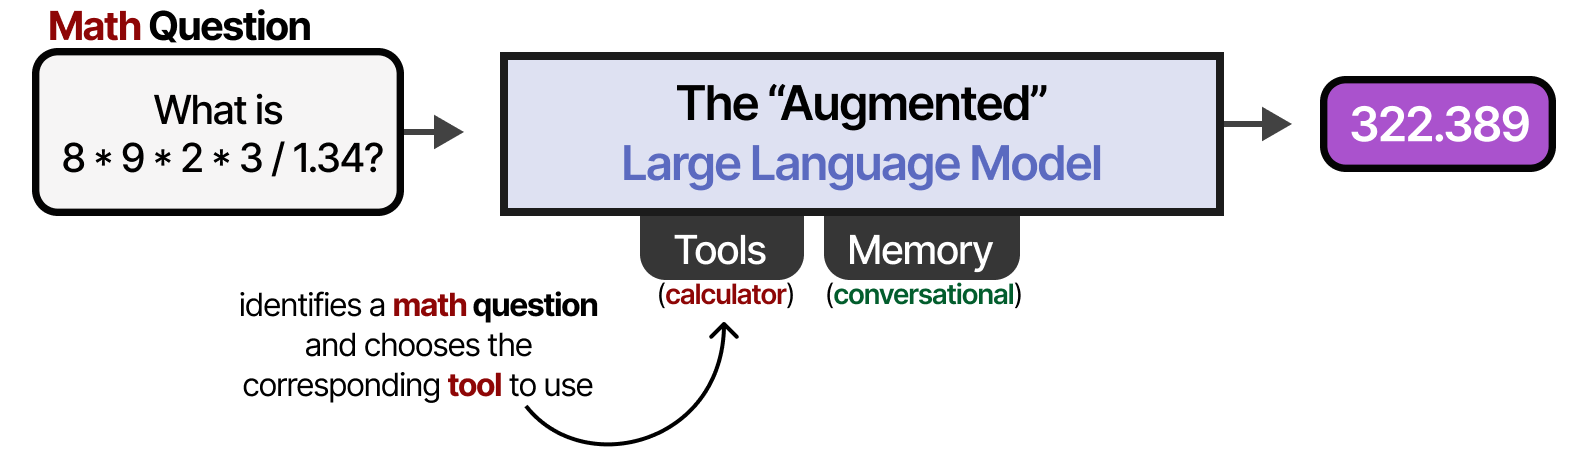
\includegraphics[width=0.8\linewidth,keepaspectratio]{aiagents94}
		
        {\tiny (Ref: A Visual Guide to Reasoning LLMs - Maarten Grootendorst)}
        \end{center}
    \end{column}
\end{columns}
\end{frame}


%%%%%%%%%%%%%%%%%%%%%%%%%%%%%%%%%%%%%%%%%%%%%%%%%%%%%%%%%%%%%%%%%%%%%%%%%%%%%%%%%%
\begin{frame}[fragile]\frametitle{What Even Is an AI Agent?}


\begin{columns}
    \begin{column}[T]{0.6\linewidth}
        \begin{center}
        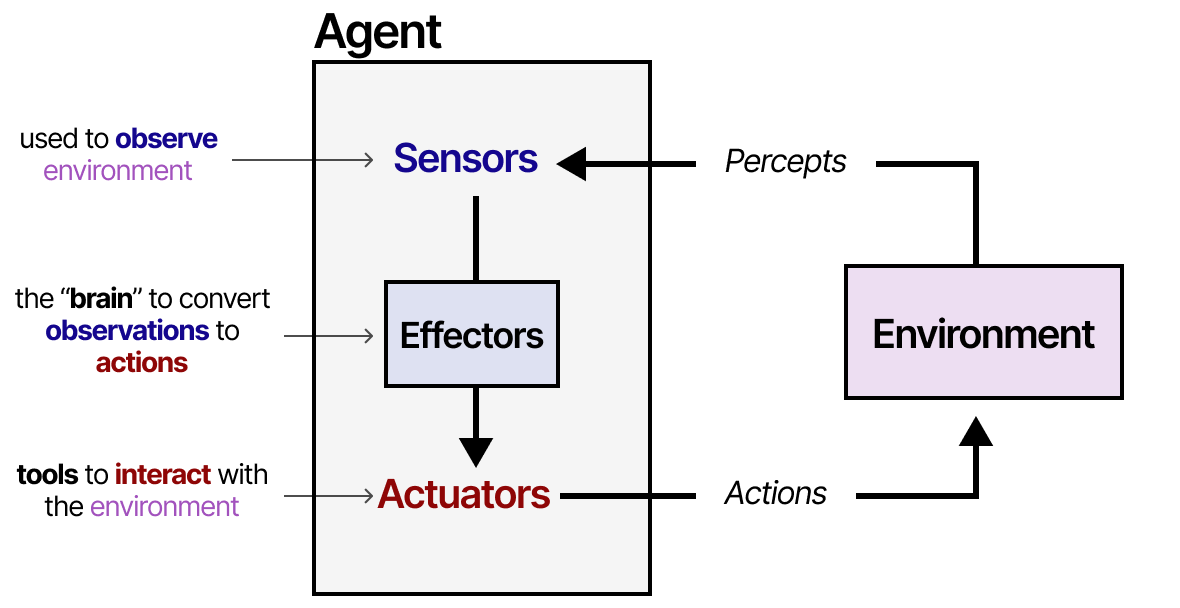
\includegraphics[width=0.8\linewidth,keepaspectratio]{aiagents95}

		
        {\tiny (Ref: A Visual Guide to Reasoning LLMs - Maarten Grootendorst)}
        \end{center}

    \end{column}
    \begin{column}[T]{0.4\linewidth}
        \begin{center}
        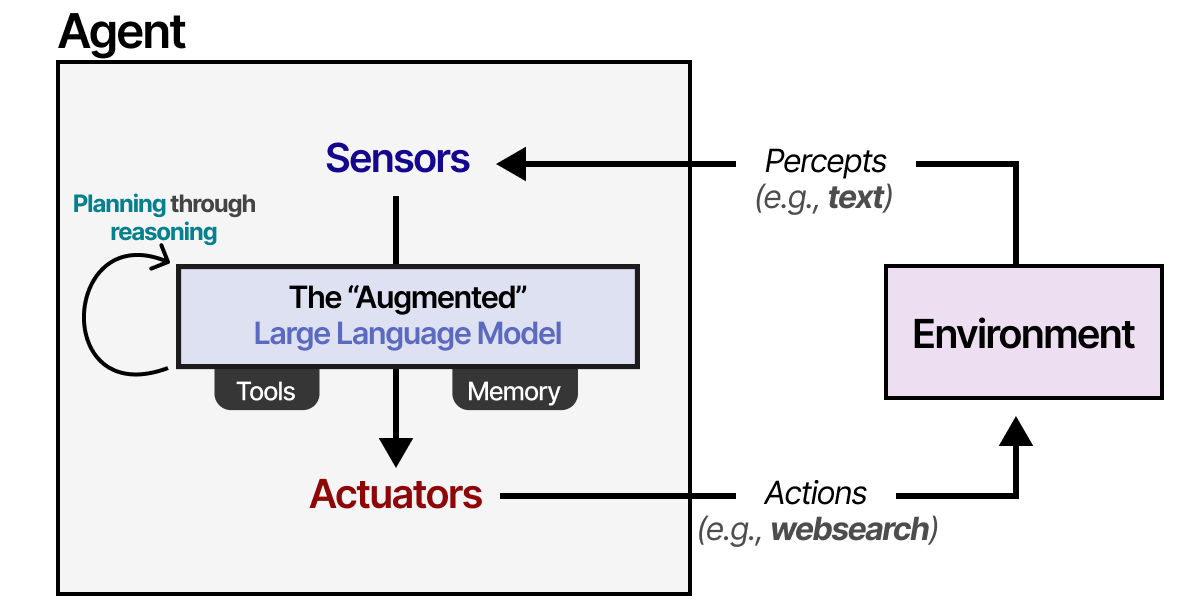
\includegraphics[width=0.8\linewidth,keepaspectratio]{aiagents96}

		
        {\tiny (Ref: A Visual Guide to Reasoning LLMs - Maarten Grootendorst)}
        \end{center}
    \end{column}
  \end{columns}
  
  


\end{frame}

%%%%%%%%%%%%%%%%%%%%%%%%%%%%%%%%%%%%%%%%%%%%%%%%%%%%%%%%%%%%%%%%%%%%%%%%%%%%%%%%%%
\begin{frame}[fragile]\frametitle{What Even Is an AI Agent?}


        \begin{center}
        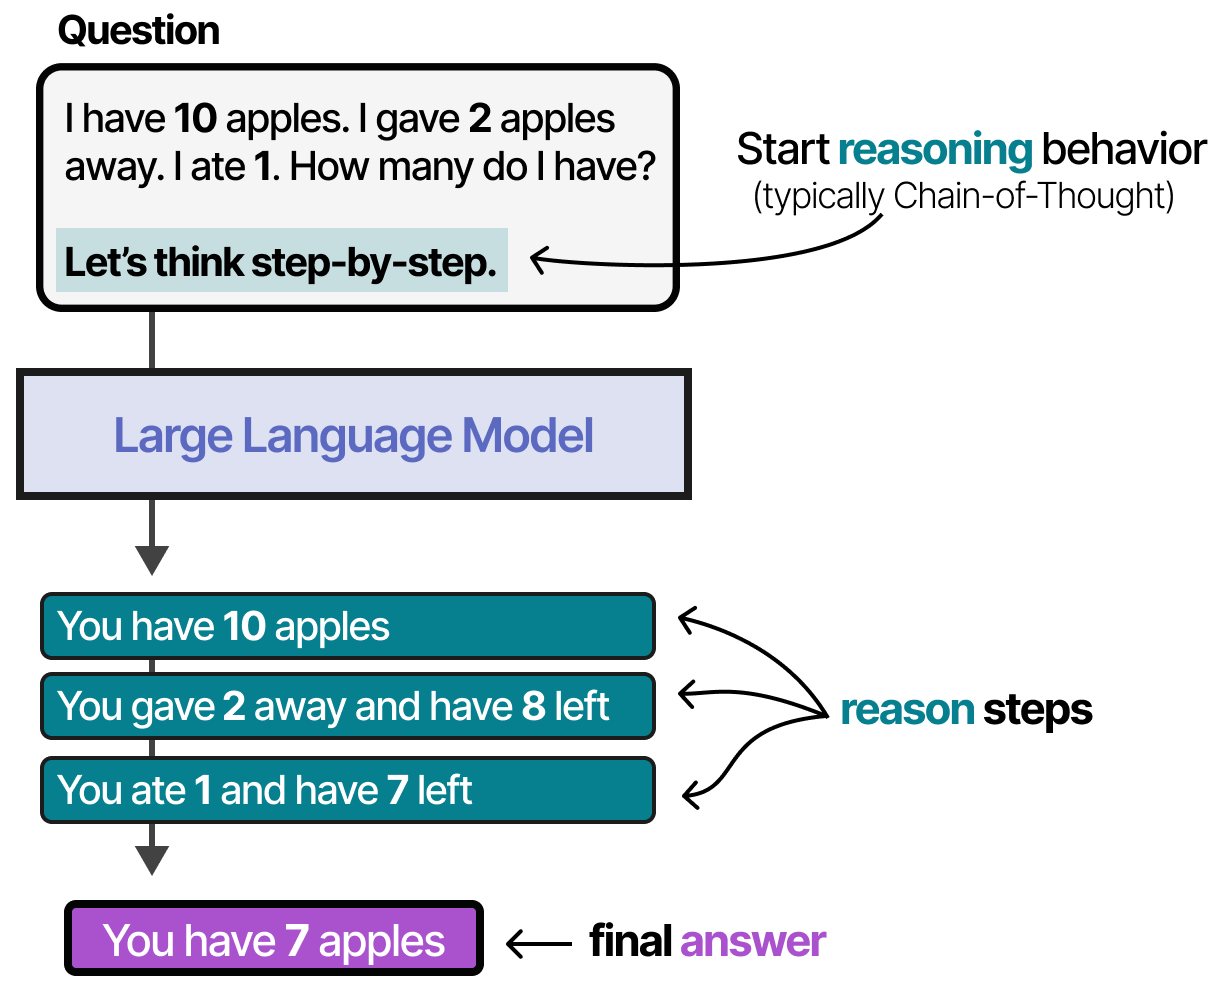
\includegraphics[width=0.8\linewidth,keepaspectratio]{aiagents97}

		
        {\tiny (Ref: A Visual Guide to Reasoning LLMs - Maarten Grootendorst)}
        \end{center}


\end{frame}


%%%%%%%%%%%%%%%%%%%%%%%%%%%%%%%%%%%%%%%%%%%%%%%%%%%%%%%%%%%%%%%%%%%%%%%%%%%%%%%%%%
\begin{frame}[fragile]\frametitle{What Even Is an AI Agent?}


\begin{columns}
    \begin{column}[T]{0.6\linewidth}
        \begin{center}
        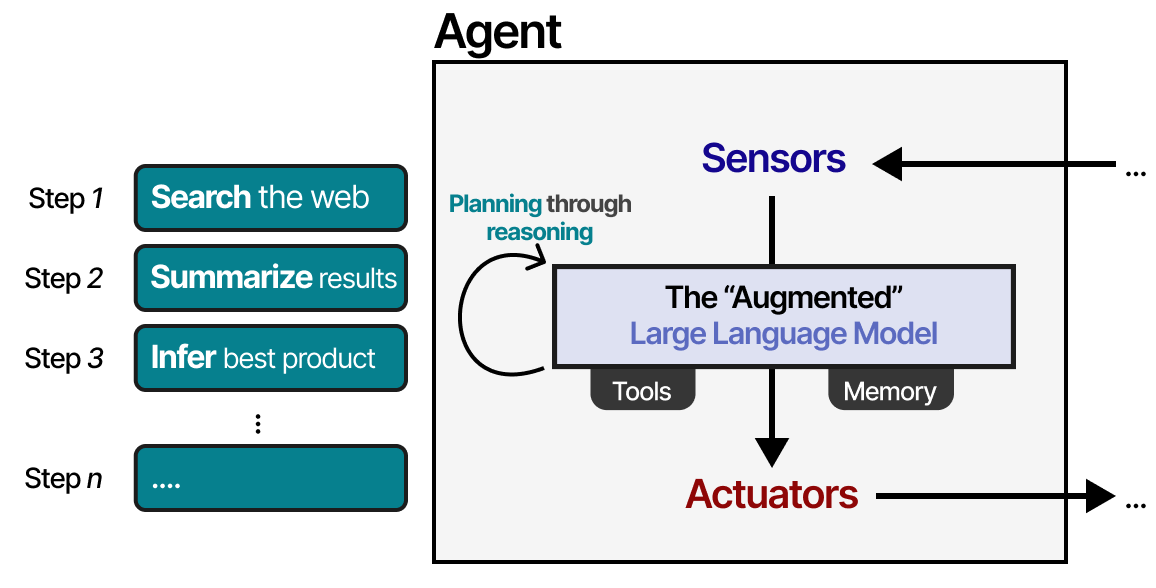
\includegraphics[width=0.8\linewidth,keepaspectratio]{aiagents98}

		
        {\tiny (Ref: A Visual Guide to Reasoning LLMs - Maarten Grootendorst)}
        \end{center}

    \end{column}
    \begin{column}[T]{0.4\linewidth}
        \begin{center}
        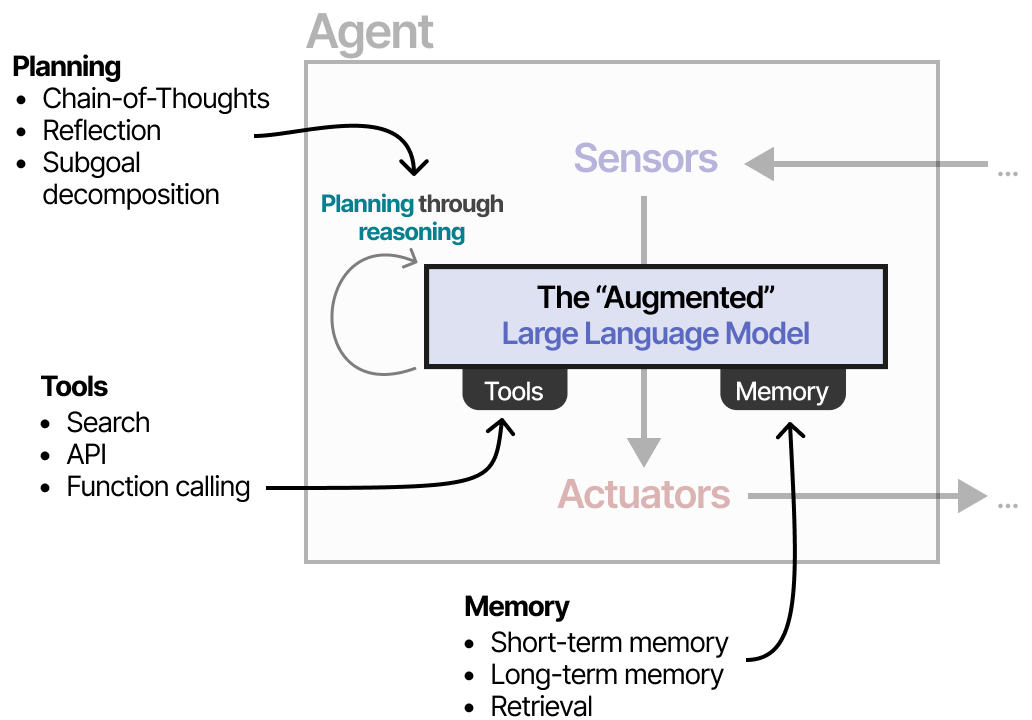
\includegraphics[width=0.8\linewidth,keepaspectratio]{aiagents99}

		
        {\tiny (Ref: A Visual Guide to Reasoning LLMs - Maarten Grootendorst)}
        \end{center}
    \end{column}
  \end{columns}

\end{frame}

%%%%%%%%%%%%%%%%%%%%%%%%%%%%%%%%%%%%%%%%%%%%%%%%%%%%%%%%%%%%%%%%%%%%%%%%%%%%%%%%%%
\begin{frame}[fragile]\frametitle{What Even Is an AI Agent?}


        \begin{center}
        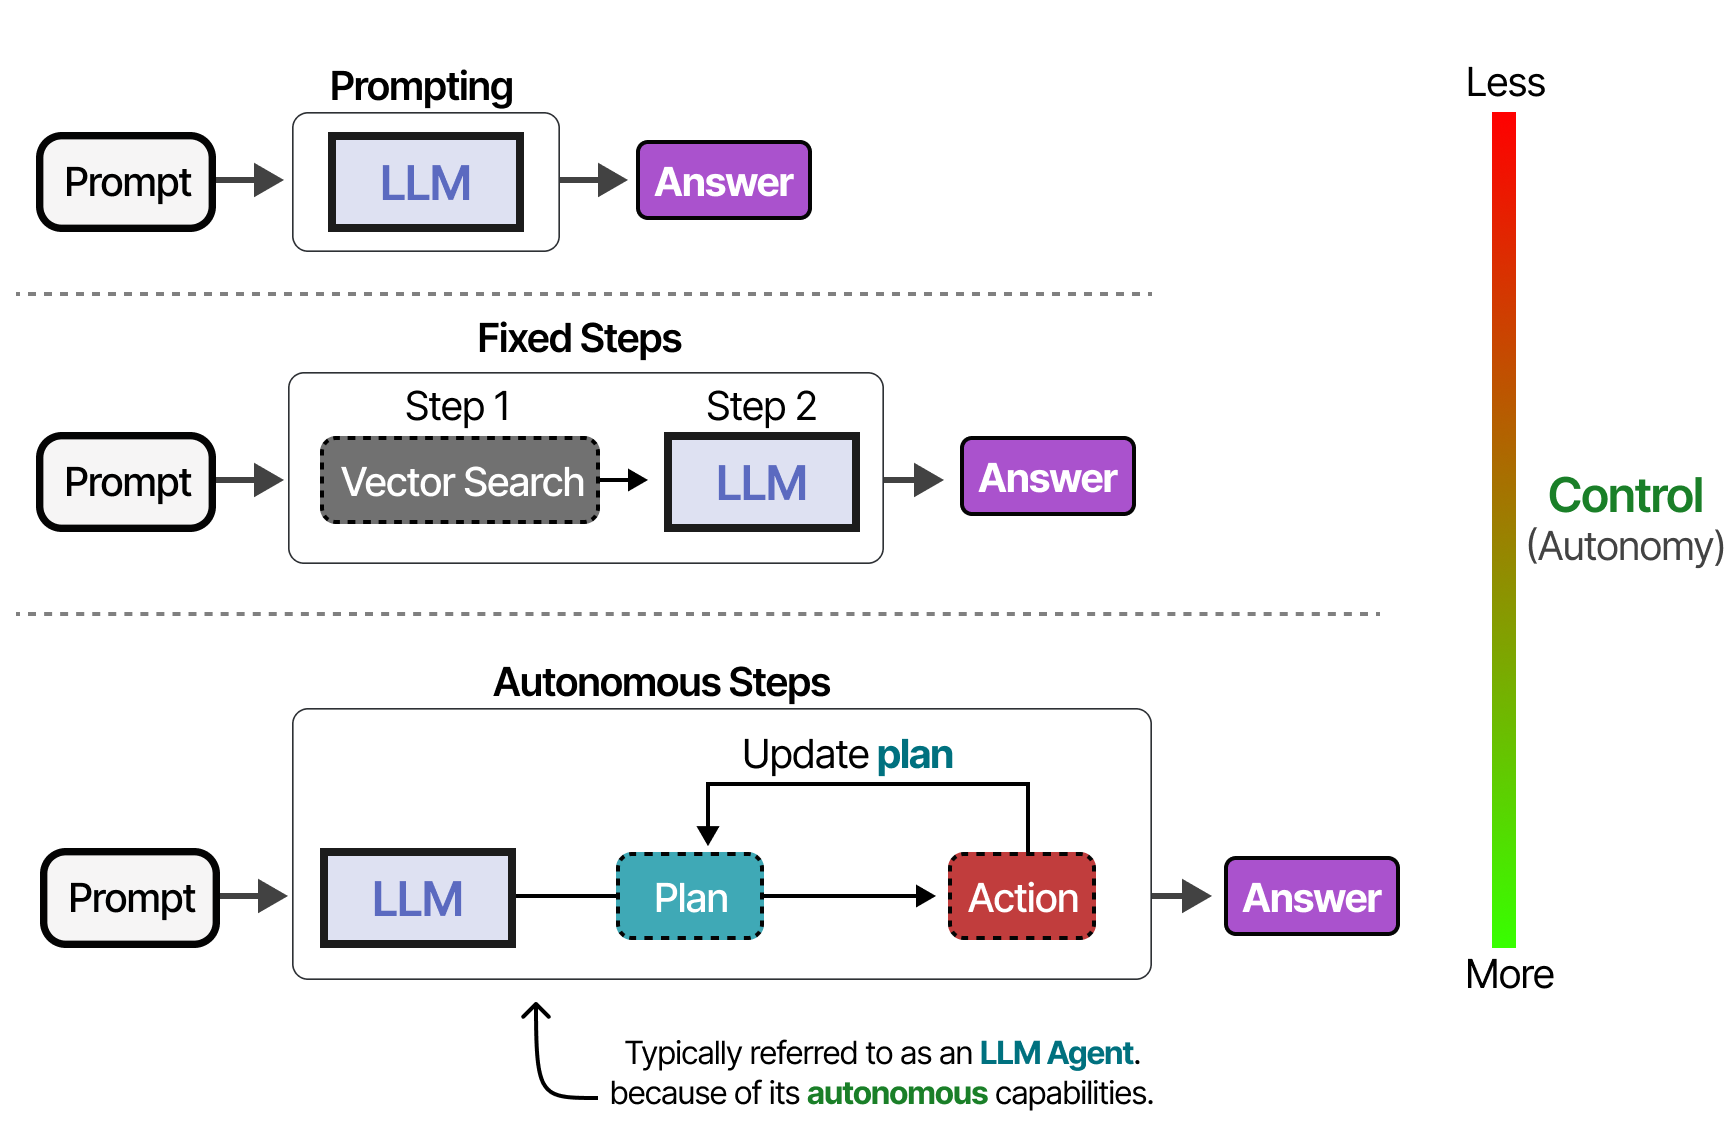
\includegraphics[width=0.8\linewidth,keepaspectratio]{aiagents100}

		
        {\tiny (Ref: A Visual Guide to Reasoning LLMs - Maarten Grootendorst)}
        \end{center}


\end{frame}

%%%%%%%%%%%%%%%%%%%%%%%%%%%%%%%%%%%%%%%%%%%%%%%%%%%%%%%%%%%
\begin{frame}[fragile]\frametitle{What Even Is an AI Agent?}
No widely accepted definition exists, but here's a practical one:

\begin{columns}
    \begin{column}[T]{0.6\linewidth}
		\begin{itemize}
			\item \textbf{Generative AI:} Great at understanding and generating content
			\item \textbf{Agentic AI:} Goes further, understands, generates content, \textbf{and performs actions}
		\end{itemize}

    \end{column}
    \begin{column}[T]{0.4\linewidth}
        \begin{center}
        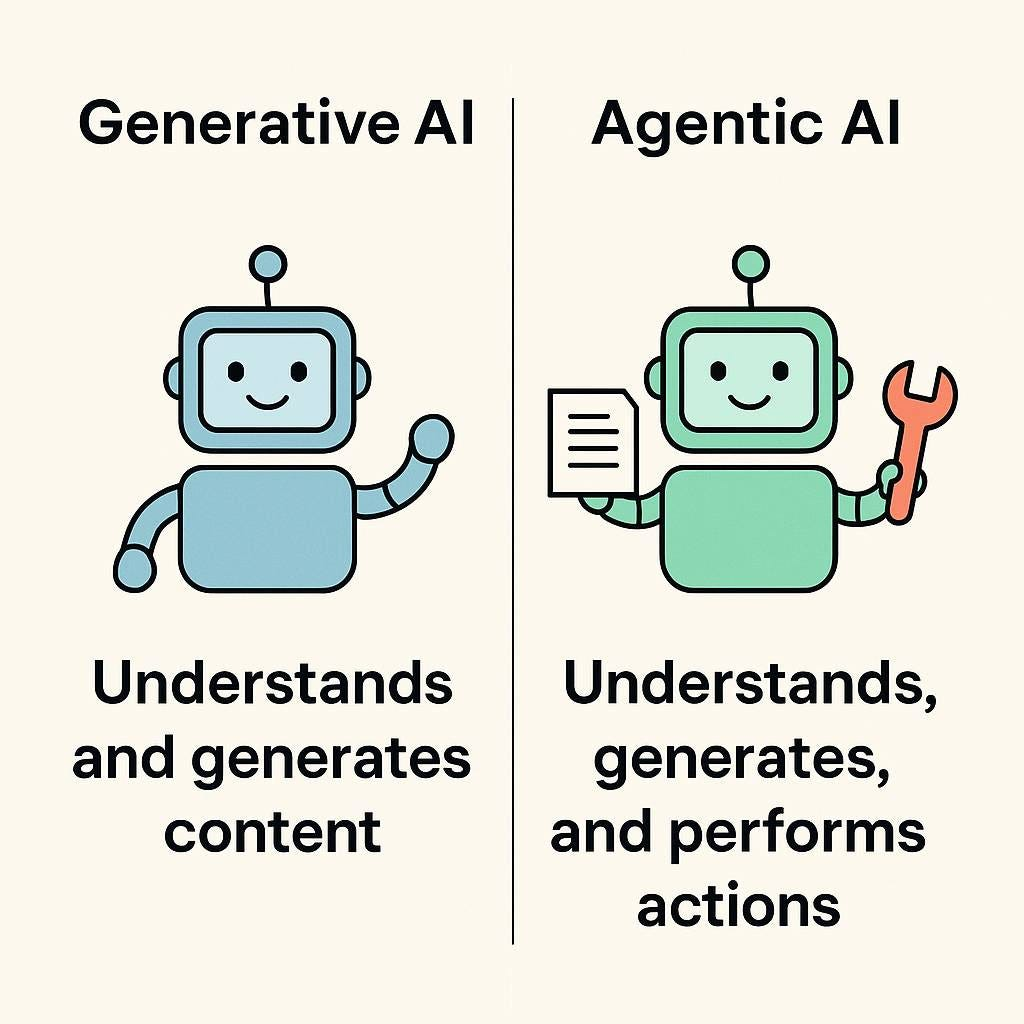
\includegraphics[width=\linewidth,keepaspectratio]{aiagents1}
		
		{\tiny (Ref: Agentic AI For Everyone - Aish \& Kiriti)}
        \end{center}
    \end{column}
  \end{columns}
  
The key differentiator is the ability to \textbf{take action}, not just respond  
\end{frame}

%%%%%%%%%%%%%%%%%%%%%%%%%%%%%%%%%%%%%%%%%%%%%%%%%%%%%%%%%%%%%%%%%%%%%%%%%%%%%%%%%%
\begin{frame}[fragile]\frametitle{The Evolution of AI Capabilities}
\begin{itemize}
    \item \textbf{Traditional Programming:} Needed code to operate
    \item \textbf{Traditional ML:} Needed feature engineering
    \item \textbf{Deep Learning:} Needed task-specific training
    \item \textbf{ChatGPT (2022):} Could reason across tasks without training
    \begin{itemize}
        \item Zero-shot learning (no examples needed)
        \item In-context learning (understands from instructions)
    \end{itemize}
    \item \textbf{Agents (2024):} Can actually \textbf{do things}, not just talk
\end{itemize}
\end{frame}

%%%%%%%%%%%%%%%%%%%%%%%%%%%%%%%%%%%%%%%%%%%%%%%%%%%%%%%%%%%%%%%%%%%%%%%%%%%%%%%%%%
\begin{frame}[fragile]\frametitle{Why Does "Taking Action" Matter?}
\begin{itemize}
    \item In 2022, ChatGPT was revolutionary because AI felt conversational
    \item By 2024, people wanted more than conversation, they wanted \textbf{execution}
    \item Examples of what users now expect:
    \begin{itemize}
        \item Instead of listing leads ? \textbf{email them directly}
        \item Instead of summarizing docs ? \textbf{file and create workflow tasks}
        \item Instead of suggesting products ? \textbf{customize landing pages}
    \end{itemize}
    \item This shift from \textbf{information} to \textbf{action} defines the agent era
\end{itemize}
\end{frame}

%%%%%%%%%%%%%%%%%%%%%%%%%%%%%%%%%%%%%%%%%%%%%%%%%%%%%%%%%%%%%%%%%%%%%%%%%%%%%%%%%%
\begin{frame}[fragile]\frametitle{How Do Agents Take Action?}
\begin{itemize}
    \item The magic lies in \textbf{tools} and \textbf{function calling}
    \item Agents are paired with APIs, plugins, or external systems
    \item Instead of just text responses, LLMs output structured commands:
    \begin{itemize}
        \item "Call the send\_email() function with these inputs..."
        \item "Fetch records from CRM using this query..."
        \item "Schedule a meeting for Tuesday at 2PM..."
    \end{itemize}
    \item \textbf{Mental model:} LLM = brain, Tools = hands
    \item Without tools, agents just talk. With tools, they act.
\end{itemize}
\end{frame}


%%%%%%%%%%%%%%%%%%%%%%%%%%%%%%%%%%%%%%%%%%%%%%%%%%%%%%%%%%%
\begin{frame}[fragile]\frametitle{Defining AI Agents with an example}

      \begin{itemize}
		\item Planning a trip involves many complex tasks
		\item Point A: Just discussing the trip
		\item Point B: All bookings and itinerary ready
		\item AI Agents aim to take you from A to B
		\item First idea: Agent adds value by saving time/money
      \end{itemize}

		\begin{center}
		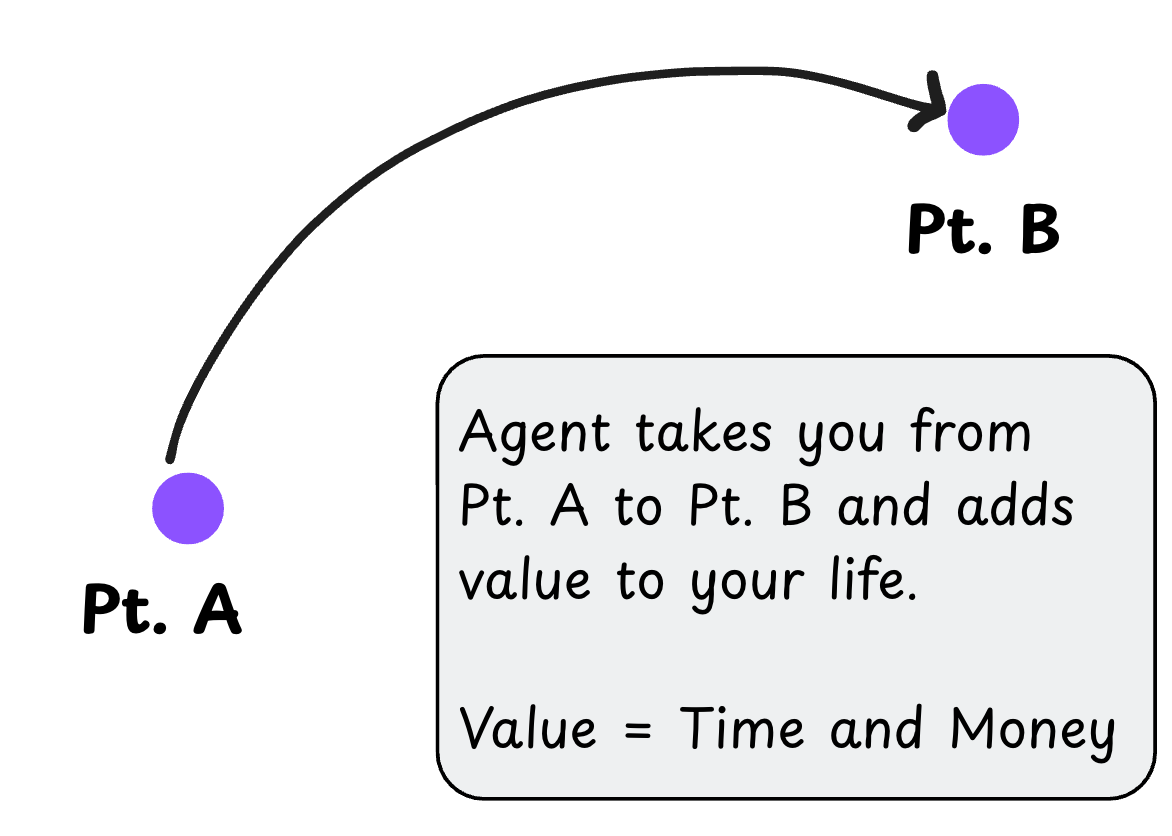
\includegraphics[width=0.6\linewidth,keepaspectratio]{aiagents25}
		
		{\tiny (Ref: Vizuara AI Agents Bootcamp)}
		\end{center}	

\end{frame}

%%%%%%%%%%%%%%%%%%%%%%%%%%%%%%%%%%%%%%%%%%%%%%%%%%%%%%%%%%%
\begin{frame}[fragile]\frametitle{Evolving Definition of Agents}

      \begin{itemize}
		\item Not all tools from A to B are agents (e.g., cars)
		\item Agents must plan and make decisions
		\item Second definition includes decision-making ability
		\item Example: Choosing flights based on budget
		\item Planning daily itinerary needs contextual judgment
      \end{itemize}

		\begin{center}
		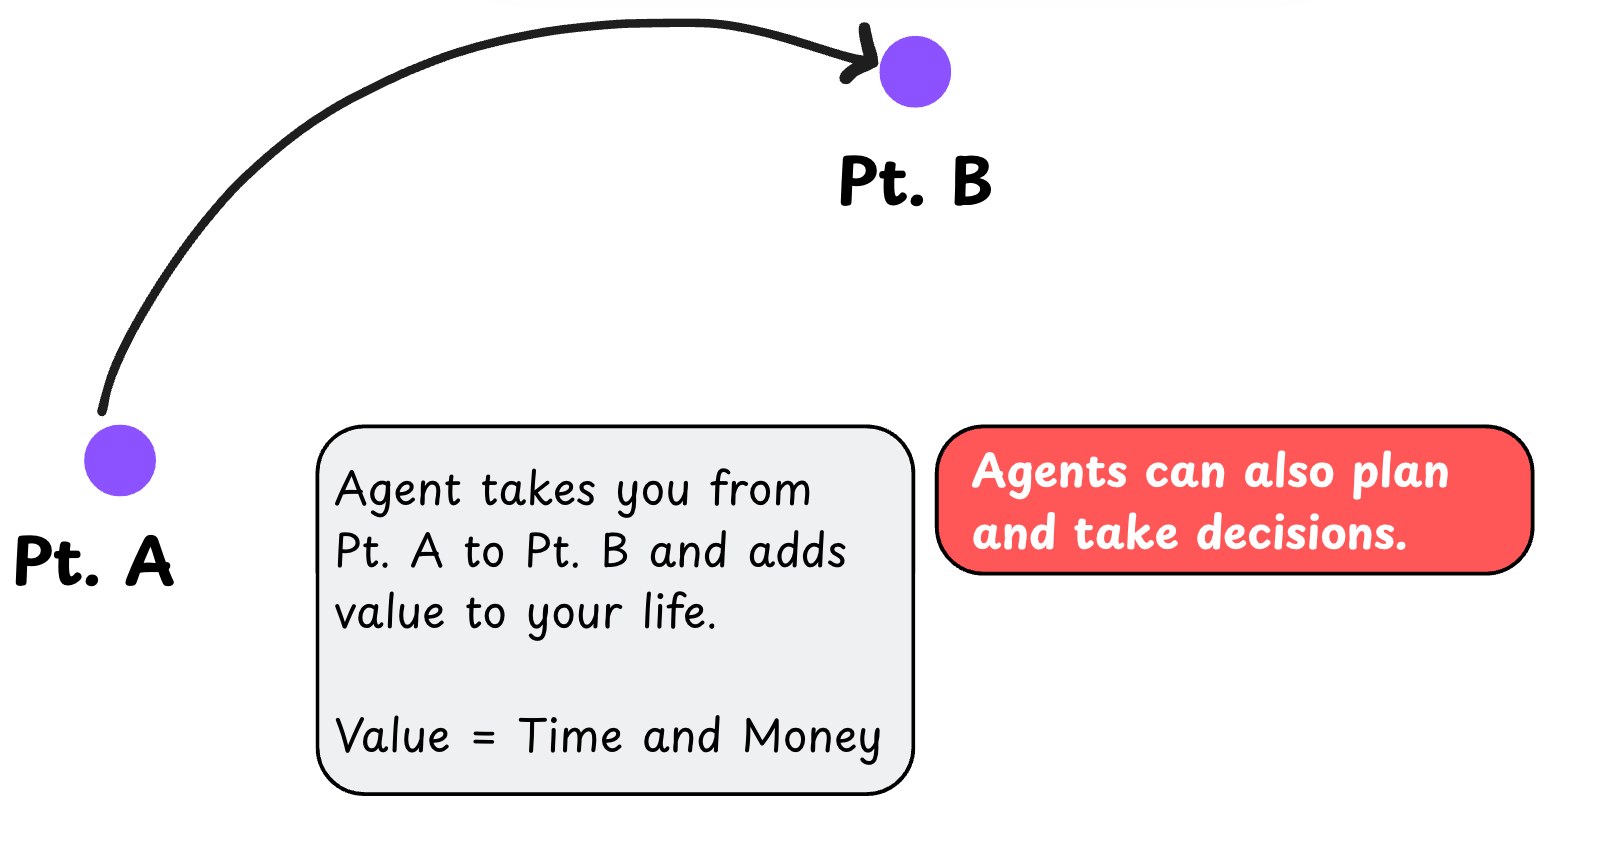
\includegraphics[width=0.6\linewidth,keepaspectratio]{aiagents26}
		
		{\tiny (Ref: Vizuara AI Agents Bootcamp)}
		\end{center}	

\end{frame}

%%%%%%%%%%%%%%%%%%%%%%%%%%%%%%%%%%%%%%%%%%%%%%%%%%%%%%%%%%%
\begin{frame}[fragile]\frametitle{Agents Need Tools}

      \begin{itemize}
        \item Even self-driving cars plan but are not agents
        \item Agents need access to external tools
        \item Tools = Access to services (e.g., Gmail, Booking)
        \item Agents perform tasks using these tools
        \item Third definition adds tool access to capabilities
      \end{itemize}

		\begin{center}
		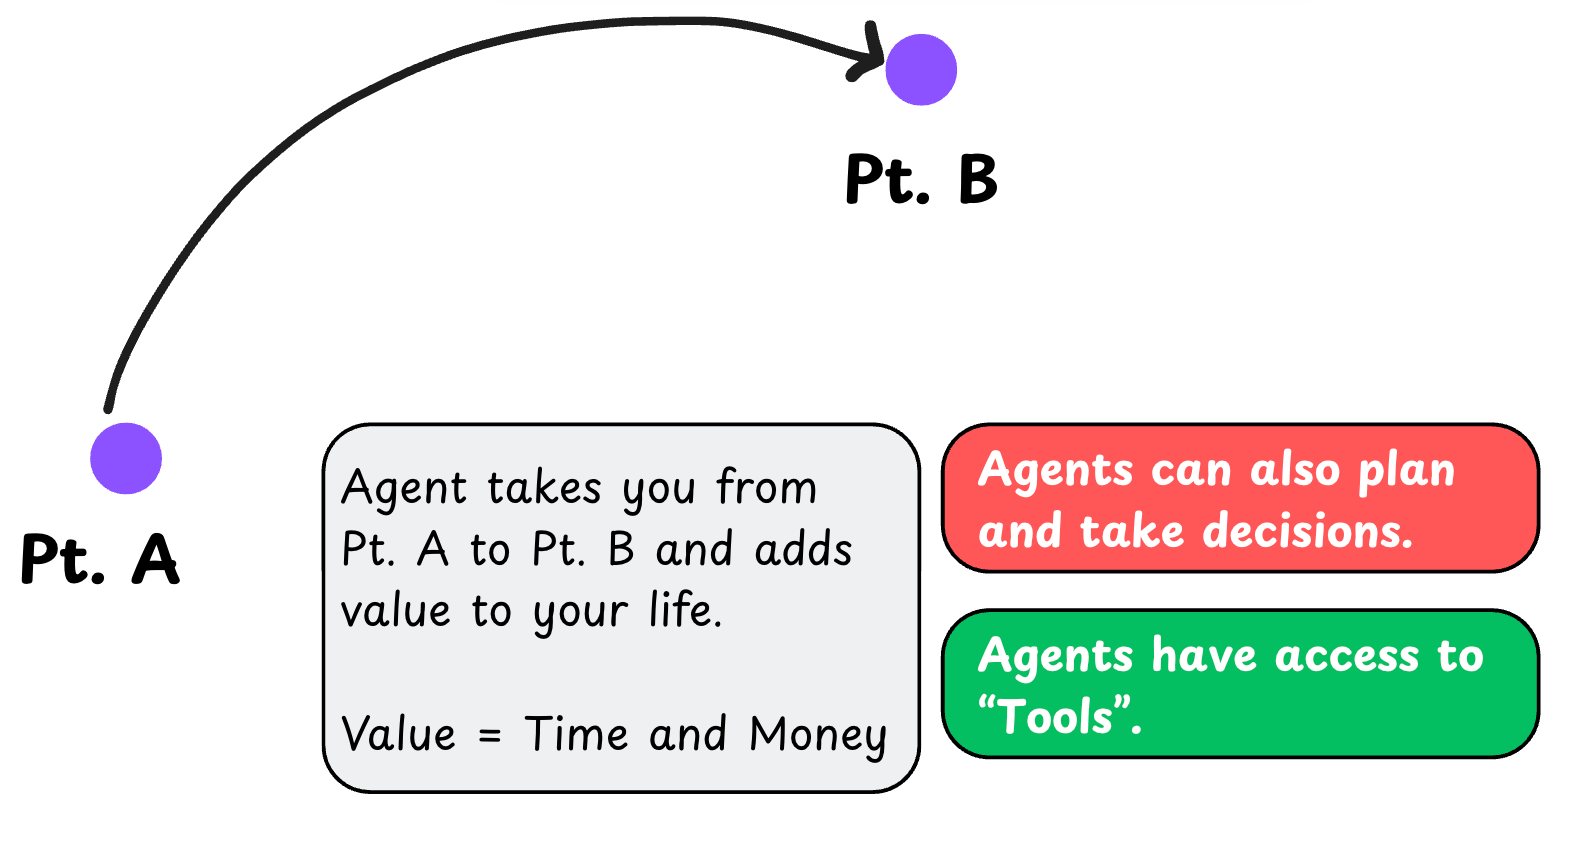
\includegraphics[width=0.6\linewidth,keepaspectratio]{aiagents27}
		
		{\tiny (Ref: Vizuara AI Agents Bootcamp)}
		\end{center}	

\end{frame}

%%%%%%%%%%%%%%%%%%%%%%%%%%%%%%%%%%%%%%%%%%%%%%%%%%%%%%%%%%%
\begin{frame}[fragile]\frametitle{Rise of LLMs in Agents}

      \begin{itemize}
        \item Transformers (2017) enabled powerful LLMs
        \item LLMs understand and generate human language
        \item Agents use LLMs for reasoning and planning
        \item LLMs enable understanding of webpages and writing emails
        \item Fourth definition: Agents are LLMs with tools and planning ability
      \end{itemize}

		\begin{center}
		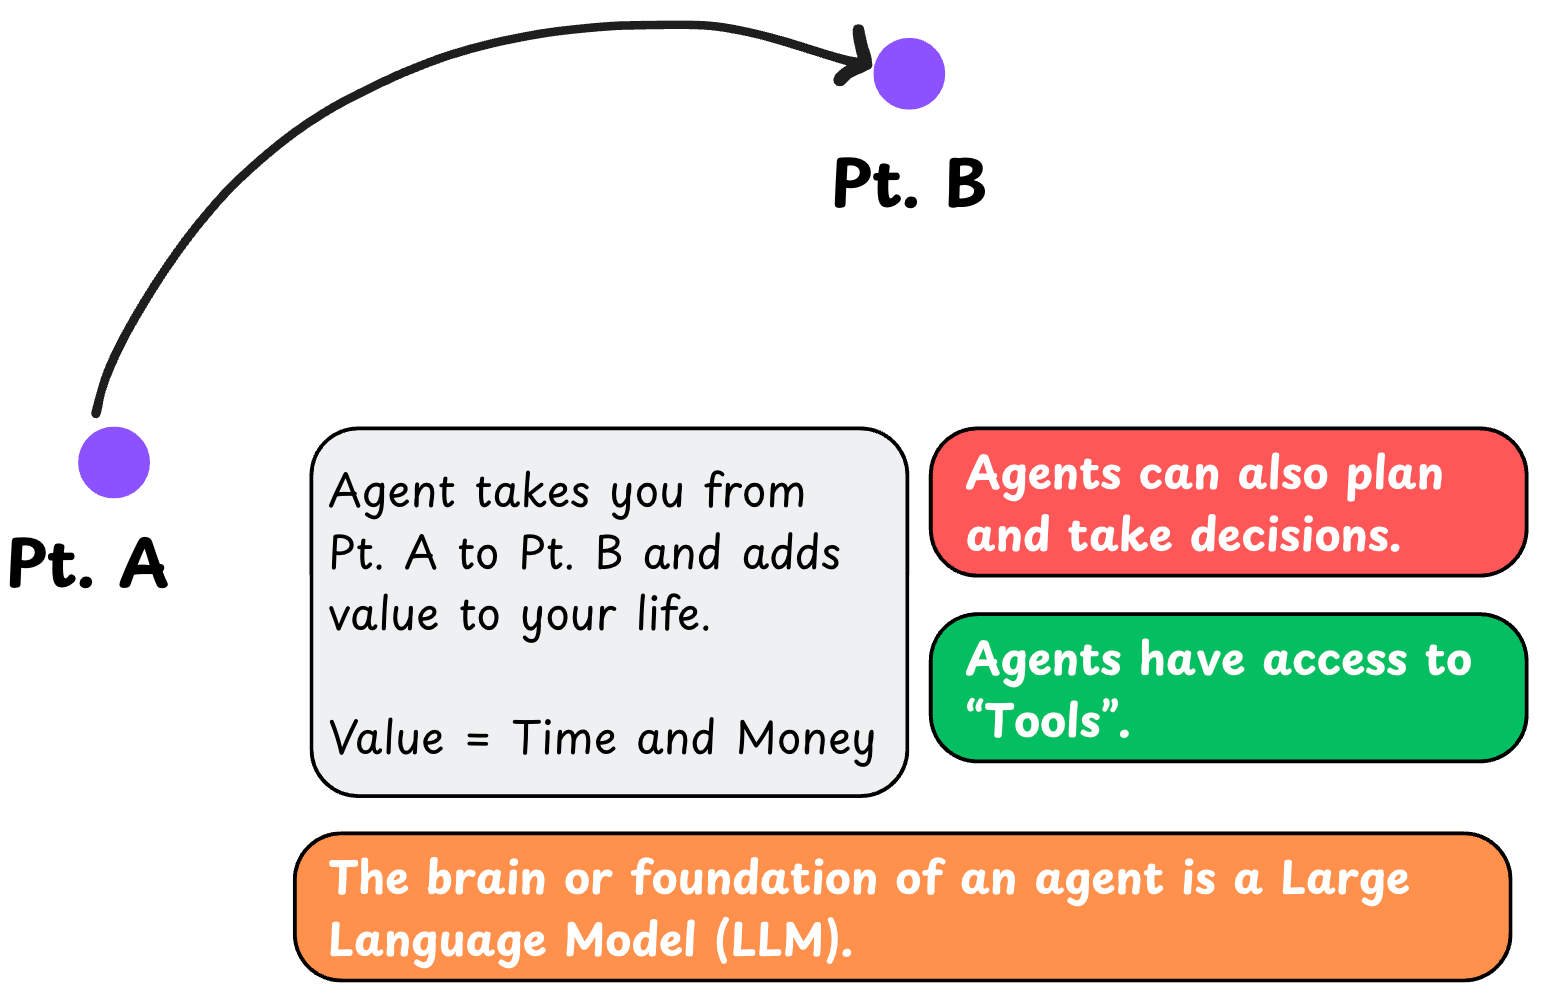
\includegraphics[width=0.6\linewidth,keepaspectratio]{aiagents28}
		
		{\tiny (Ref: Vizuara AI Agents Bootcamp)}
		\end{center}	

\end{frame}



%%%%%%%%%%%%%%%%%%%%%%%%%%%%%%%%%%%%%%%%%%%%%%%%%%%%%%%%%%%%%%%%%%%%%%%%%%%%%%%%%%
\begin{frame}[fragile]\frametitle{What Is an Agent? (Technical Definition)}
\begin{itemize}
    \item Agent acts and takes you from one state to another, providing value through workflow automation
    \item Based on ReAct paradigm: \textbf{Reasoning + Acting}
    \item Key capabilities:
    \begin{itemize}
        \item Can plan and make decisions
        \item Has access to tools (search APIs, booking, email, etc.)
        \item Interacts with external environments and other agents
        \item Maintains memory of conversations and actions
        \item May include human-in-the-loop for safety
    \end{itemize}
    \item Agents existed since the 1950s but are now effective because of LLMs
\end{itemize}
\end{frame}


%%%%%%%%%%%%%%%%%%%%%%%%%%%%%%%%%%%%%%%%%%%%%%%%%%%%%%%%%%%%%%%%%%%%%%%%%%%%%%%%%%
\begin{frame}[fragile]\frametitle{Two Ways to Define Agents}
\begin{columns}
    \begin{column}[T]{0.5\linewidth}
        \textbf{Technical View:}
        \begin{itemize}
            \item LLM (brain)
            \item + Tools (hands)
            \item + Planning (strategy)
            \item + Memory (context)
            \item + State management
        \end{itemize}
    \end{column}
    \begin{column}[T]{0.5\linewidth}
        \textbf{Business View:}
        \begin{itemize}
            \item Systems that complete tasks end-to-end
            \item Focus on outcomes, not components
            \item Solve real-world problems
            \item Provide measurable value
        \end{itemize}
    \end{column}
\end{columns}

\vspace{0.5cm}
\textbf{Important:} Today's agents are \textbf{engineering wrappers} around AI models, the intelligence comes from the LLMs, agents help act on that intelligence.
\end{frame}


%%%%%%%%%%%%%%%%%%%%%%%%%%%%%%%%%%%%%%%%%%%%%%%%%%%%%%%%%%%
\begin{frame}[fragile]\frametitle{Final Definition of Agents}

      \begin{itemize}
        \item Agents can learn from feedback and environment
        \item Agents interact with tools, humans, and websites
        \item They improve with experience (memory)
        \item Fifth definition: LLMs + Tools + Planning + Learning
        \item Agents evolve over time via memory and feedback
      \end{itemize}

		\begin{center}
		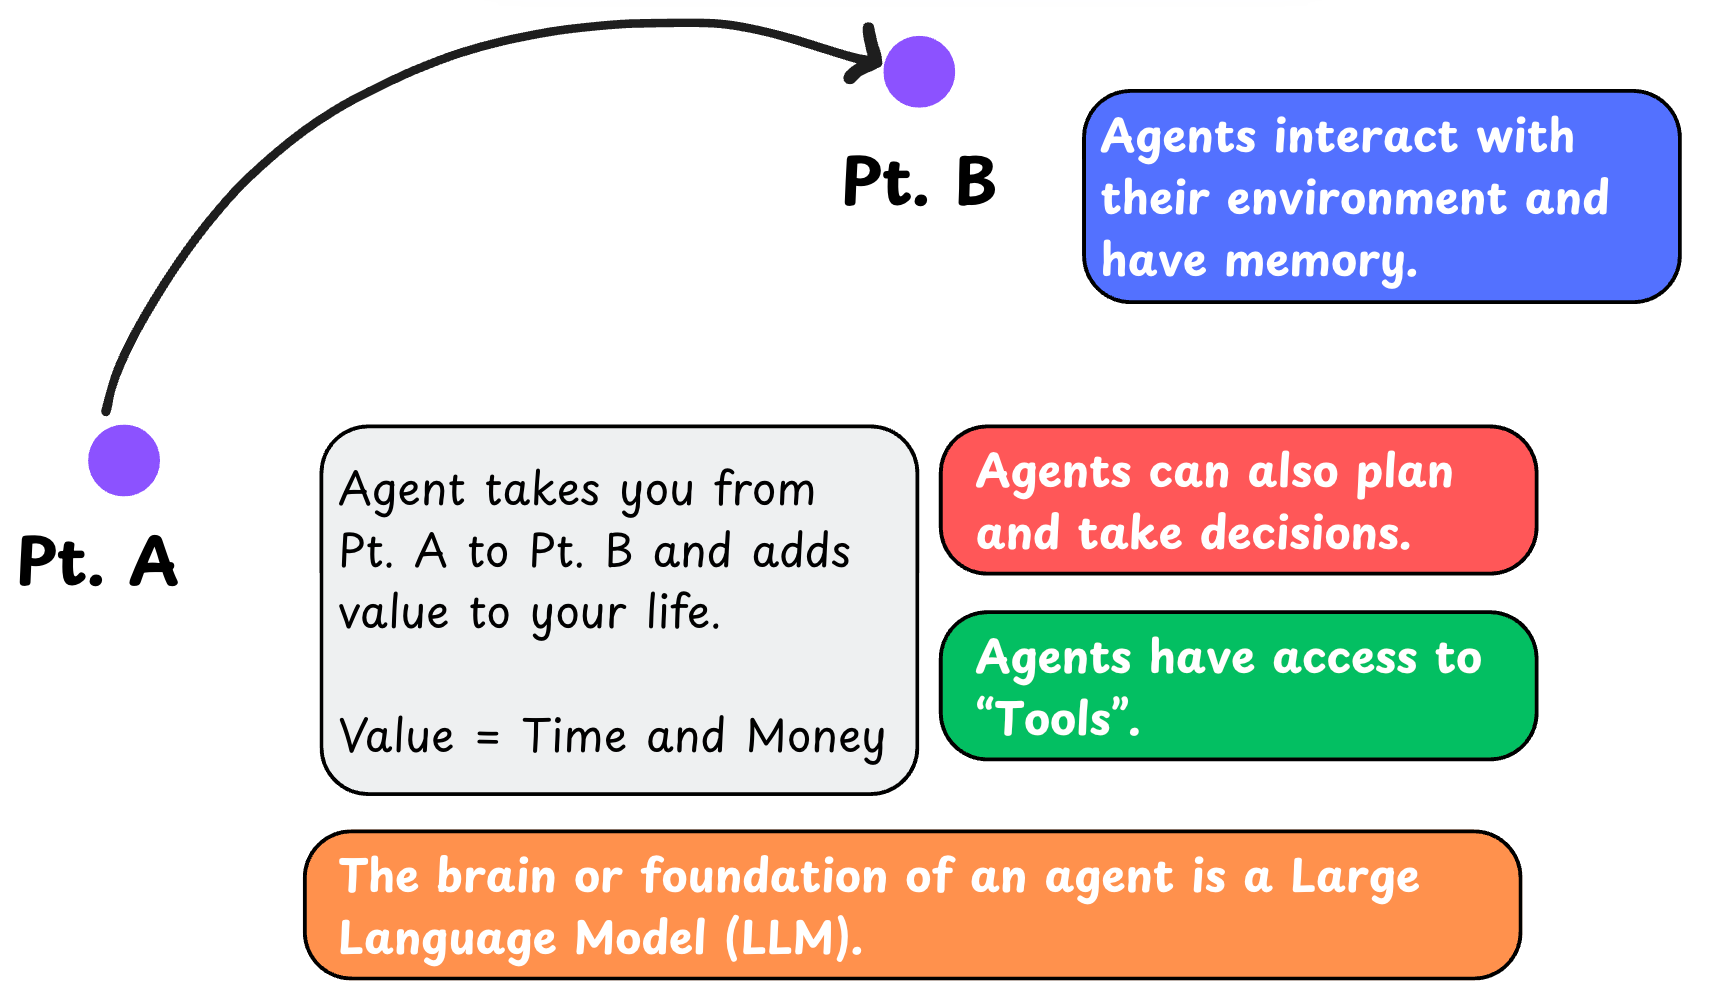
\includegraphics[width=0.6\linewidth,keepaspectratio]{aiagents29}
		
		{\tiny (Ref: Vizuara AI Agents Bootcamp)}
		\end{center}	

\end{frame}

%%%%%%%%%%%%%%%%%%%%%%%%%%%%%%%%%%%%%%%%%%%%%%%%%%%%%%%%%%%
\begin{frame}[fragile]\frametitle{Understanding Agency}

      \begin{itemize}
        \item Agency = Level of autonomy an agent has
        \item Low agency → less value
        \item High agency → high value
        \item More autonomous agents can handle complex tasks
        \item Agency is key to measuring agent usefulness
      \end{itemize}

		\begin{center}
		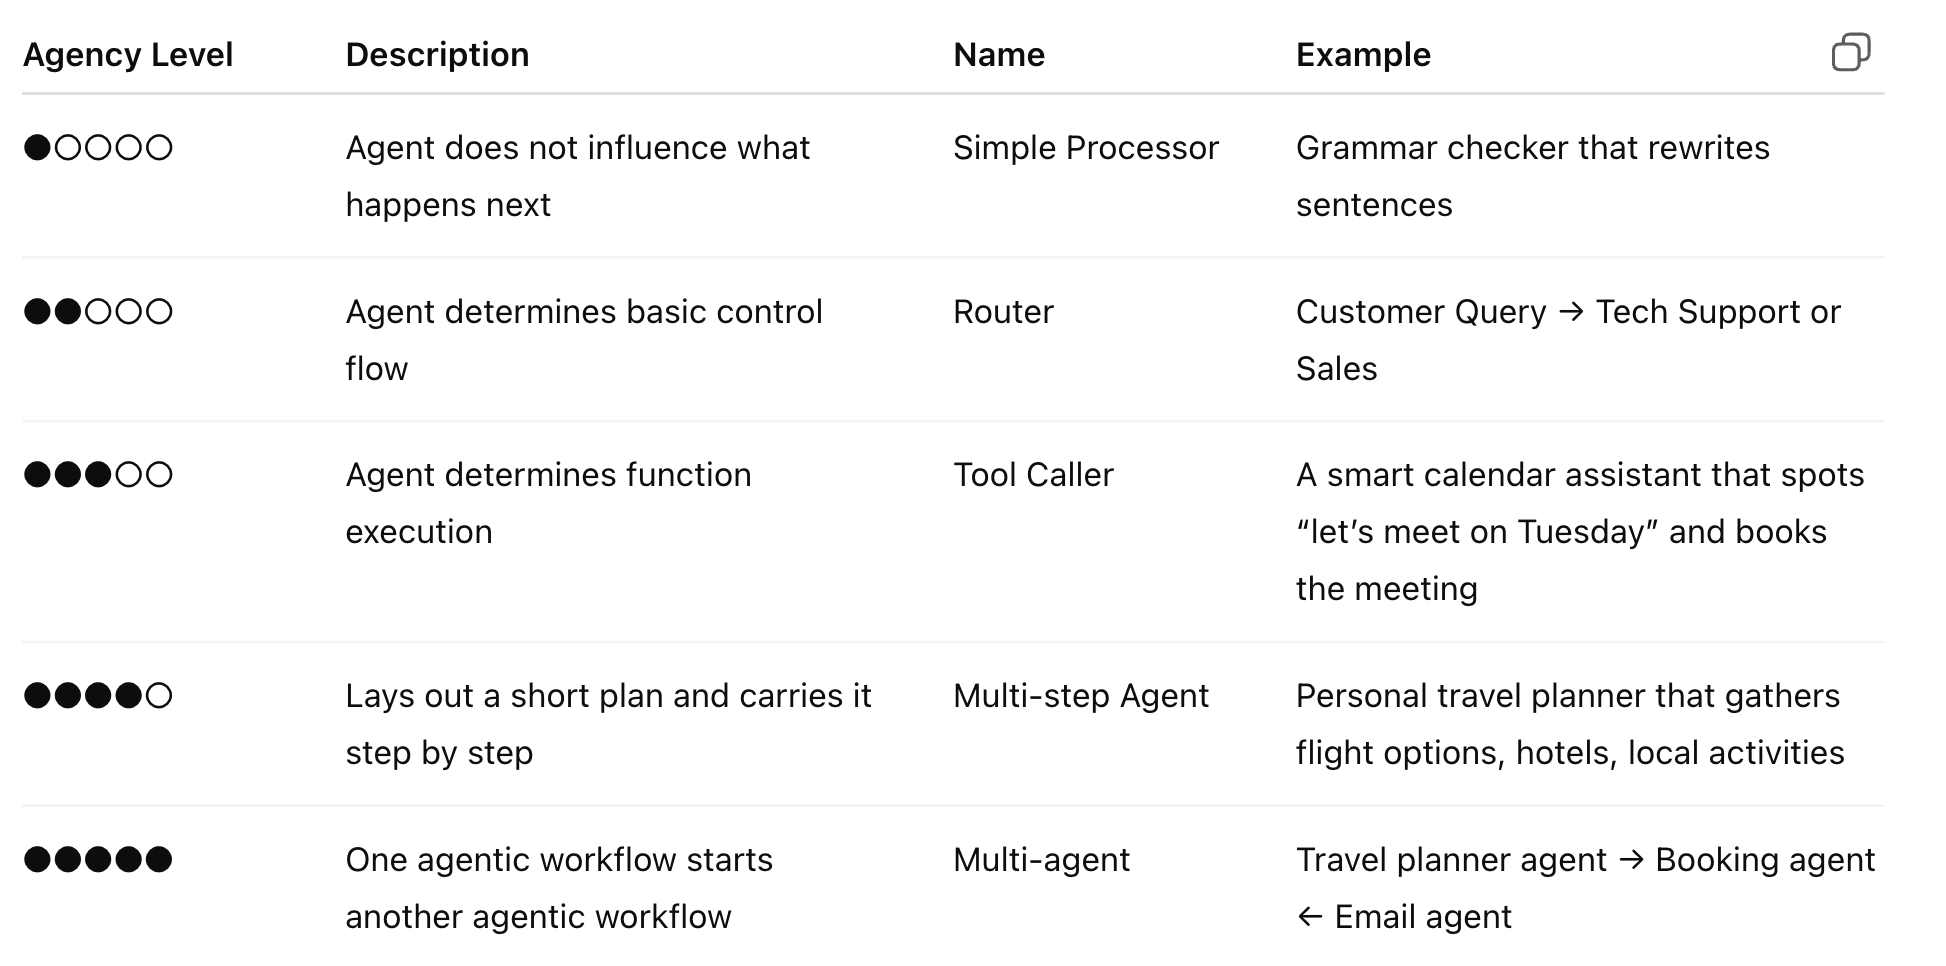
\includegraphics[width=0.8\linewidth,keepaspectratio]{aiagents30}
		
		{\tiny (Ref: Vizuara AI Agents Bootcamp)}
		\end{center}	

\end{frame}

%%%%%%%%%%%%%%%%%%%%%%%%%%%%%%%%%%%%%%%%%%%%%%%%%%%%%%%%%%%
\begin{frame}[fragile]\frametitle{Papers that Shaped AI Agents}

      \begin{itemize}
        \item Core research papers laid the foundation
        \item Introduced key frameworks and architectures
        \item Sparked recent boom in agent development
        \item Include Transformer and Agentic frameworks
        \item Major driving force in LLM-based agent systems
      \end{itemize}

		\begin{center}
		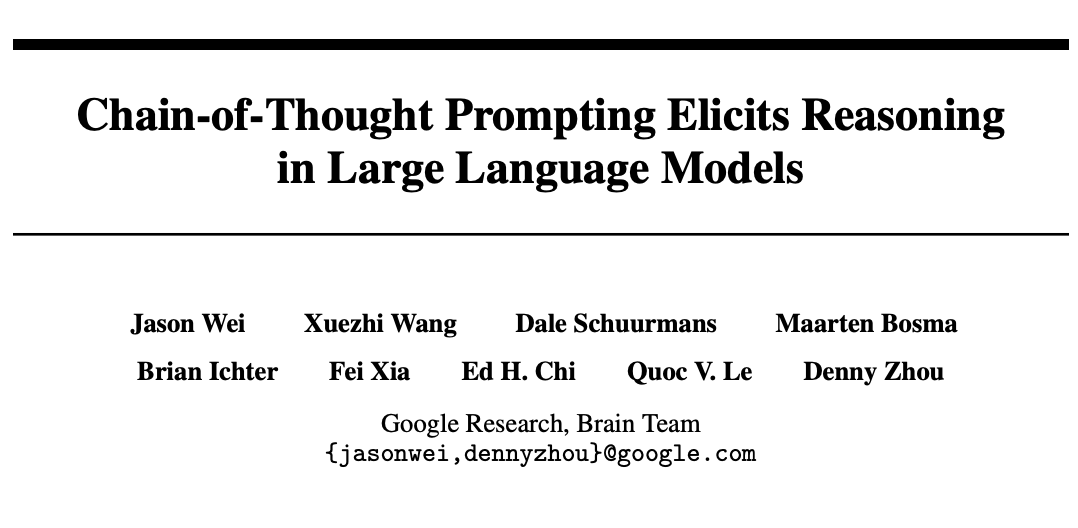
\includegraphics[width=0.45\linewidth,keepaspectratio]{aiagents31}
		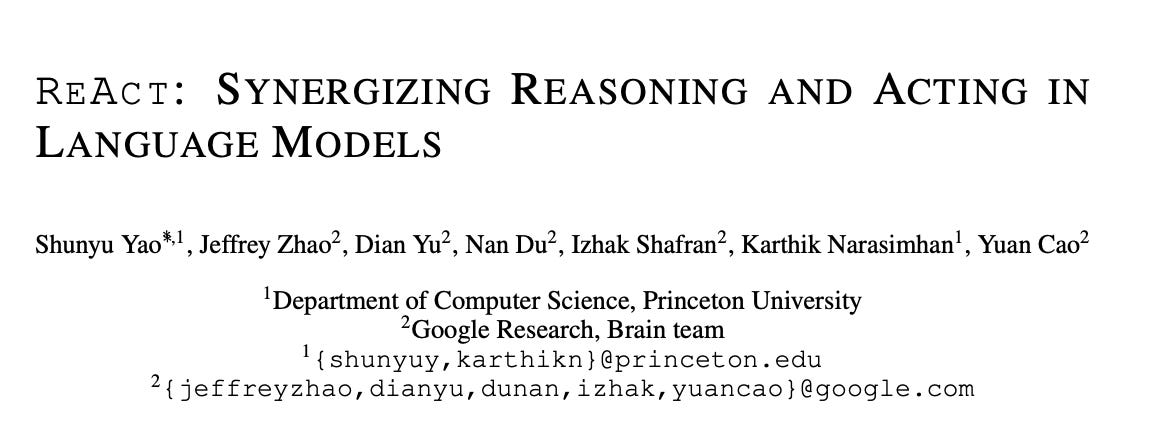
\includegraphics[width=0.45\linewidth,keepaspectratio]{aiagents32}
		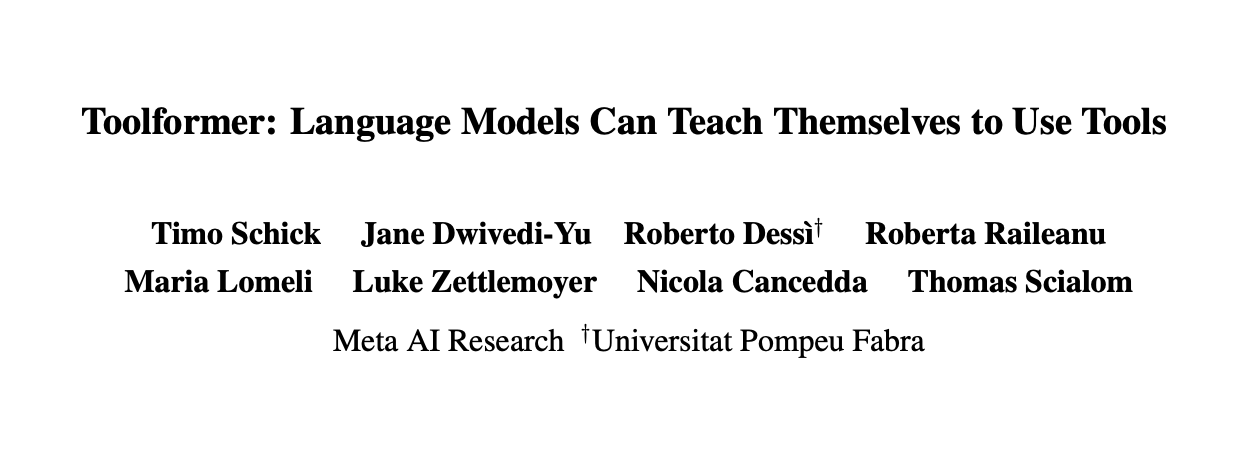
\includegraphics[width=0.45\linewidth,keepaspectratio]{aiagents33}
		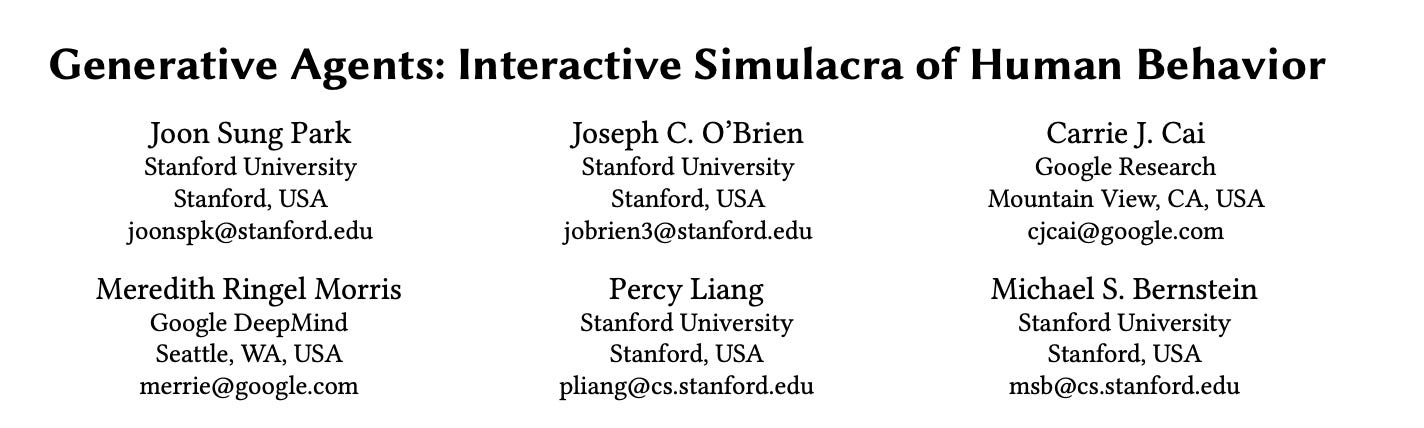
\includegraphics[width=0.45\linewidth,keepaspectratio]{aiagents34}
		
		{\tiny (Ref: Vizuara AI Agents Bootcamp)}
		\end{center}	
 
\end{frame}

%%%%%%%%%%%%%%%%%%%%%%%%%%%%%%%%%%%%%%%%%%%%%%%%%%%%%%%%%%%%%%%%%%%%%%%%%%%%%%%%%%
\begin{frame}[fragile]\frametitle{When to Use Agents?}
    \begin{itemize}
        \item Best suited for tasks requiring flexibility and model-driven decision-making
        \item Consider tradeoffs: agents increase latency and cost for better task performance
        \item Recommended for open-ended problems with unpredictable steps
        \item Simple solutions preferred - single LLM calls with retrieval often sufficient
    \end{itemize}
\end{frame}

%%%%%%%%%%%%%%%%%%%%%%%%%%%%%%%%%%%%%%%%%%%%%%%%%%%%%%%%%%%%%%%%%%%%%%%%%%%%%%%%%%
\begin{frame}[fragile]\frametitle{Future AI Applications}
\begin{itemize}
    \item What are future AI applications like?
    \begin{itemize}
        \item \textbf{Generative:} Generate content like text and images
        \item \textbf{Agentic:} Execute complex tasks on behalf of humans
    \end{itemize}
    \item How do we empower every developer to build them?
    \begin{itemize}
        \item \textbf{Co-Pilots:} Human-AI collaboration
        \item \textbf{Autonomous:} Independent task execution
    \end{itemize}
    \item 2024 is expected to be the year of AI agents
\end{itemize}
\end{frame}


